%   PACKAGES AND CUSTOMIZATIONS  %%%%%%%%%%%%%%%%%%%%%%%%
\documentclass[12pt]{article}
\usepackage{amsmath}
\usepackage{amssymb}
\usepackage{amsthm}
\usepackage[pdfborder={0 0 0}]{hyperref}
\usepackage{graphicx}
\usepackage{caption}
\usepackage{natbib}
\usepackage{wrapfig}
\usepackage{enumitem}
\setlist[enumerate]{itemsep=0mm}
\usepackage{multirow}
\usepackage{lscape}
\usepackage{caption}
\usepackage{subcaption}
\usepackage{float}
\usepackage{hyperref}
\usepackage{tabularx}
\usepackage{rotating}
\captionsetup[subfigure]{position=top, labelfont=bf,textfont=normalfont,singlelinecheck=off,justification=raggedright}
\renewcommand{\vector}[1]{\mathbf{#1}}
\usepackage{adjustbox}
\usepackage{bm}


\newcommand{\transectAbb}{Data for each glacier are divided into lower hourglass (LH), lower circle (LC), lower midline (LM), upper hourglass (UH), upper circle (UC), upper midline (UM), and upper transect (UT).}
\newcommand{\params}{Topographic parameters are distance from centreline ($d_C$), elevation ($z$), aspect ($\alpha$), slope ($m$), northness ($N$), curvature ($\kappa$), and Sx. }
\newcommand{\boxplot}{Within each box, the mean is shown as a circle, the median as a horizontal line, the interquartile range (IQR) as a coloured box, two times the IQR as dashed lines beyond the box, and outliers as single points. }
\newcommand{\boxMatlab}{Red line indicates median, blue box shows first quantiles, bars indicate minimum and maximum values (excluding outliers), and red crosses show outliers, which are defined as being outside of the range of 1.5 times the quartiles (approximately $\pm2.7\sigma$). }
\newcommand{\topomap}{Arrows indicate glacier flow direction and black dots show snow depth sampling locations. }
\newcommand{\blackdots}{Observed SWE values are overlain on the maps. }


\begin{document}

Background to kriging -> literature use 
Background on regression kriging 
Specific package

What to do with lower and upper bounds?

Kriged swe
Kriged residuals and added to BMA

Final R2 value and rmse comparison of kriged, BMA, RK -> all density options?
sweKRIG vs SWE
sweRK vs SWE


Appendix -> manual for kriging 


%% Next time
- background writing
- describe figures
- calculate R2, rmse, residuals hist for RK
- table of kriging model params 



\section{Kriging}

\subsection{Background}


\begin{figure}
	\centering
	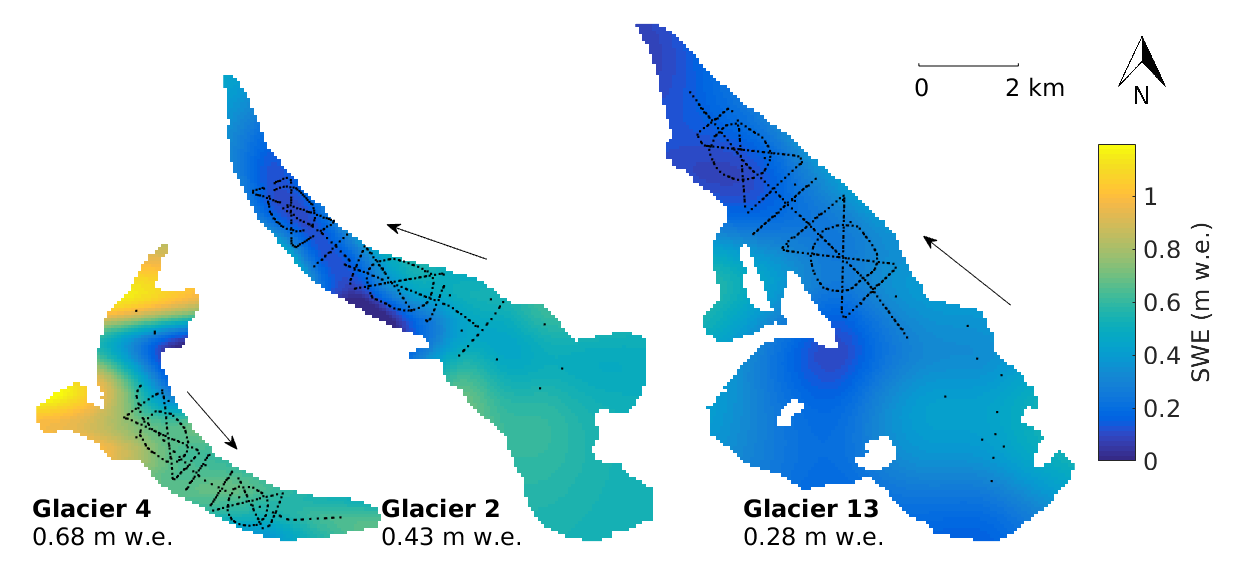
\includegraphics[width = \textwidth]{sweKriged.png}\\
	\caption{Estimated SWE found by kriging measured SWE. \topomap}
	\label{fig:sweKRIGING}
\end{figure}


\begin{table}[]
\centering
\caption{Nugget (m w.e.) estimated for SWE data using maximum log likelihood?? in DiceKriging package.}
\label{tab:sweKrigNugget}
\begin{tabular}{c|ccc}
\textbf{\begin{tabular}[c]{@{}c@{}}Density\\ Option\end{tabular}} & \textbf{Glacier 4} & \textbf{Glacier 2} & \textbf{Glacier 13} \\ \hline
\textbf{S1} & 0.015 & 0.004 & 0.004 \\
\textbf{F1} & 0.013 & 0.003 & 0.003 \\ \hline
\textbf{S2} & 0.009 & 0.004 & 0.004 \\
\textbf{F2} & 0.009 & 0.003 & 0.003 \\ \hline
\textbf{S3} & 0.016 & 0.004 & 0.005 \\
\textbf{F3} & 0.017 & 0.002 & 0.003 \\ \hline
\textbf{S4} & 0.014 & 0.004 & 0.004 \\
\textbf{F4} & 0.009 & 0.002 & 0.003
\end{tabular}
\end{table}





\begin{figure}
	\centering
	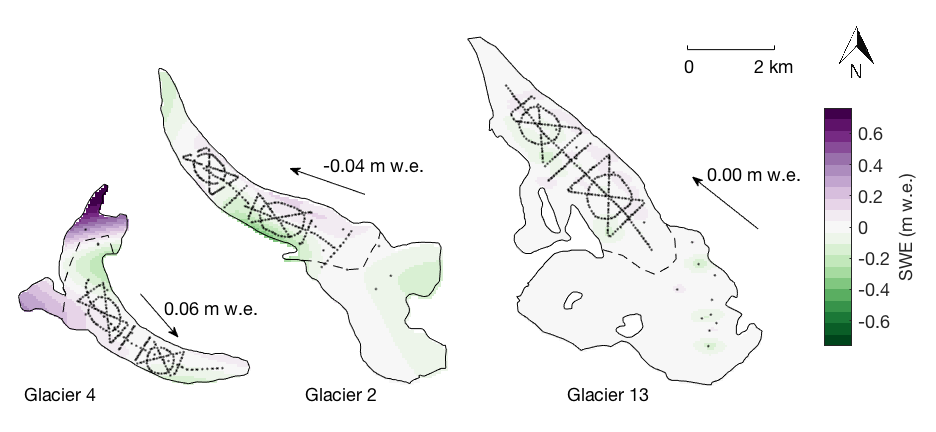
\includegraphics[width = \textwidth]{residualsKriged.png}\\
	\caption{Estimate of BMA residuals found by kriging. \topomap}
	\label{fig:residualsKRIGING}
\end{figure}

\begin{figure}
	\centering
	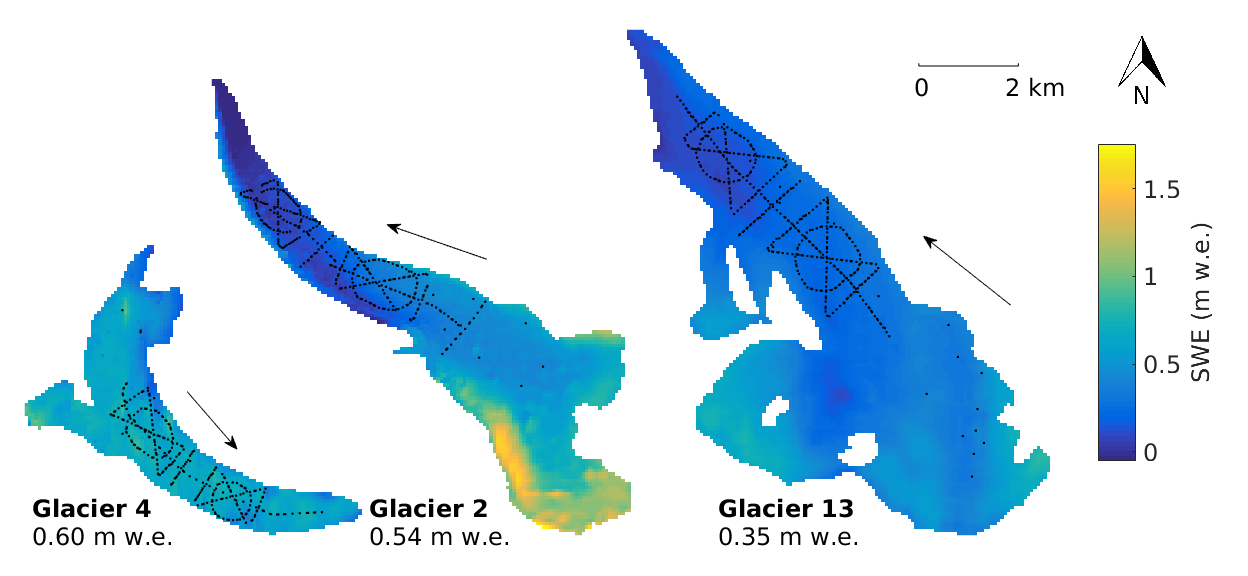
\includegraphics[width = \textwidth]{RegressionKriging.png}\\
	\caption{Estimated SWE found by adding the estimated residuals (kriging) to the estimated SWE found using BMA. \topomap}
	\label{fig:Regression-Kriging}
\end{figure}


\section{Kriging software}
\label{sec:KrigingMethods}
Data kriging was executed using the DiceKriging package in R (??). The function \texttt{KrigingR()} computes the kriged surface of input data through DiceKriging, as well as the upper and lower confidence intervals, the cross-validated (leave one out) estimates of SWE, as well as parameters that describe the kriging model fit (nugget, maximum log likelihood and mean constant). 



\end{document} 